% Options for packages loaded elsewhere
\PassOptionsToPackage{unicode}{hyperref}
\PassOptionsToPackage{hyphens}{url}
%
\documentclass[
]{article}
\usepackage{lmodern}
\usepackage{amssymb,amsmath}
\usepackage{ifxetex,ifluatex}
\ifnum 0\ifxetex 1\fi\ifluatex 1\fi=0 % if pdftex
  \usepackage[T1]{fontenc}
  \usepackage[utf8]{inputenc}
  \usepackage{textcomp} % provide euro and other symbols
\else % if luatex or xetex
  \usepackage{unicode-math}
  \defaultfontfeatures{Scale=MatchLowercase}
  \defaultfontfeatures[\rmfamily]{Ligatures=TeX,Scale=1}
\fi
% Use upquote if available, for straight quotes in verbatim environments
\IfFileExists{upquote.sty}{\usepackage{upquote}}{}
\IfFileExists{microtype.sty}{% use microtype if available
  \usepackage[]{microtype}
  \UseMicrotypeSet[protrusion]{basicmath} % disable protrusion for tt fonts
}{}
\makeatletter
\@ifundefined{KOMAClassName}{% if non-KOMA class
  \IfFileExists{parskip.sty}{%
    \usepackage{parskip}
  }{% else
    \setlength{\parindent}{0pt}
    \setlength{\parskip}{6pt plus 2pt minus 1pt}}
}{% if KOMA class
  \KOMAoptions{parskip=half}}
\makeatother
\usepackage{xcolor}
\IfFileExists{xurl.sty}{\usepackage{xurl}}{} % add URL line breaks if available
\IfFileExists{bookmark.sty}{\usepackage{bookmark}}{\usepackage{hyperref}}
\hypersetup{
  pdftitle={Simple 3-state Markov model in R},
  pdfauthor={The DARTH workgroup},
  hidelinks,
  pdfcreator={LaTeX via pandoc}}
\urlstyle{same} % disable monospaced font for URLs
\usepackage[margin=1in]{geometry}
\usepackage{color}
\usepackage{fancyvrb}
\newcommand{\VerbBar}{|}
\newcommand{\VERB}{\Verb[commandchars=\\\{\}]}
\DefineVerbatimEnvironment{Highlighting}{Verbatim}{commandchars=\\\{\}}
% Add ',fontsize=\small' for more characters per line
\usepackage{framed}
\definecolor{shadecolor}{RGB}{248,248,248}
\newenvironment{Shaded}{\begin{snugshade}}{\end{snugshade}}
\newcommand{\AlertTok}[1]{\textcolor[rgb]{0.94,0.16,0.16}{#1}}
\newcommand{\AnnotationTok}[1]{\textcolor[rgb]{0.56,0.35,0.01}{\textbf{\textit{#1}}}}
\newcommand{\AttributeTok}[1]{\textcolor[rgb]{0.77,0.63,0.00}{#1}}
\newcommand{\BaseNTok}[1]{\textcolor[rgb]{0.00,0.00,0.81}{#1}}
\newcommand{\BuiltInTok}[1]{#1}
\newcommand{\CharTok}[1]{\textcolor[rgb]{0.31,0.60,0.02}{#1}}
\newcommand{\CommentTok}[1]{\textcolor[rgb]{0.56,0.35,0.01}{\textit{#1}}}
\newcommand{\CommentVarTok}[1]{\textcolor[rgb]{0.56,0.35,0.01}{\textbf{\textit{#1}}}}
\newcommand{\ConstantTok}[1]{\textcolor[rgb]{0.00,0.00,0.00}{#1}}
\newcommand{\ControlFlowTok}[1]{\textcolor[rgb]{0.13,0.29,0.53}{\textbf{#1}}}
\newcommand{\DataTypeTok}[1]{\textcolor[rgb]{0.13,0.29,0.53}{#1}}
\newcommand{\DecValTok}[1]{\textcolor[rgb]{0.00,0.00,0.81}{#1}}
\newcommand{\DocumentationTok}[1]{\textcolor[rgb]{0.56,0.35,0.01}{\textbf{\textit{#1}}}}
\newcommand{\ErrorTok}[1]{\textcolor[rgb]{0.64,0.00,0.00}{\textbf{#1}}}
\newcommand{\ExtensionTok}[1]{#1}
\newcommand{\FloatTok}[1]{\textcolor[rgb]{0.00,0.00,0.81}{#1}}
\newcommand{\FunctionTok}[1]{\textcolor[rgb]{0.00,0.00,0.00}{#1}}
\newcommand{\ImportTok}[1]{#1}
\newcommand{\InformationTok}[1]{\textcolor[rgb]{0.56,0.35,0.01}{\textbf{\textit{#1}}}}
\newcommand{\KeywordTok}[1]{\textcolor[rgb]{0.13,0.29,0.53}{\textbf{#1}}}
\newcommand{\NormalTok}[1]{#1}
\newcommand{\OperatorTok}[1]{\textcolor[rgb]{0.81,0.36,0.00}{\textbf{#1}}}
\newcommand{\OtherTok}[1]{\textcolor[rgb]{0.56,0.35,0.01}{#1}}
\newcommand{\PreprocessorTok}[1]{\textcolor[rgb]{0.56,0.35,0.01}{\textit{#1}}}
\newcommand{\RegionMarkerTok}[1]{#1}
\newcommand{\SpecialCharTok}[1]{\textcolor[rgb]{0.00,0.00,0.00}{#1}}
\newcommand{\SpecialStringTok}[1]{\textcolor[rgb]{0.31,0.60,0.02}{#1}}
\newcommand{\StringTok}[1]{\textcolor[rgb]{0.31,0.60,0.02}{#1}}
\newcommand{\VariableTok}[1]{\textcolor[rgb]{0.00,0.00,0.00}{#1}}
\newcommand{\VerbatimStringTok}[1]{\textcolor[rgb]{0.31,0.60,0.02}{#1}}
\newcommand{\WarningTok}[1]{\textcolor[rgb]{0.56,0.35,0.01}{\textbf{\textit{#1}}}}
\usepackage{graphicx,grffile}
\makeatletter
\def\maxwidth{\ifdim\Gin@nat@width>\linewidth\linewidth\else\Gin@nat@width\fi}
\def\maxheight{\ifdim\Gin@nat@height>\textheight\textheight\else\Gin@nat@height\fi}
\makeatother
% Scale images if necessary, so that they will not overflow the page
% margins by default, and it is still possible to overwrite the defaults
% using explicit options in \includegraphics[width, height, ...]{}
\setkeys{Gin}{width=\maxwidth,height=\maxheight,keepaspectratio}
% Set default figure placement to htbp
\makeatletter
\def\fps@figure{htbp}
\makeatother
\setlength{\emergencystretch}{3em} % prevent overfull lines
\providecommand{\tightlist}{%
  \setlength{\itemsep}{0pt}\setlength{\parskip}{0pt}}
\setcounter{secnumdepth}{-\maxdimen} % remove section numbering

\title{Simple 3-state Markov model in R}
\usepackage{etoolbox}
\makeatletter
\providecommand{\subtitle}[1]{% add subtitle to \maketitle
  \apptocmd{\@title}{\par {\large #1 \par}}{}{}
}
\makeatother
\subtitle{with dependency for time-since model start AND with state-residency
dependency}
\author{The DARTH workgroup}
\date{}

\begin{document}
\maketitle

Developed by the Decision Analysis in R for Technologies in Health
(DARTH) workgroup:

Fernando Alarid-Escudero, PhD (1)

Eva A. Enns, MS, PhD (2)

M.G. Myriam Hunink, MD, PhD (3,4)

Hawre J. Jalal, MD, PhD (5)

Eline M. Krijkamp, MSc (3)

Petros Pechlivanoglou, PhD (6,7)

Alan Yang, MSc (7)

In collaboration of:

\begin{enumerate}
\def\labelenumi{\arabic{enumi}.}
\tightlist
\item
  Drug Policy Program, Center for Research and Teaching in Economics
  (CIDE) - CONACyT, Aguascalientes, Mexico
\item
  University of Minnesota School of Public Health, Minneapolis, MN, USA
\item
  Erasmus MC, Rotterdam, The Netherlands
\item
  Harvard T.H. Chan School of Public Health, Boston, USA
\item
  University of Pittsburgh Graduate School of Public Health, Pittsburgh,
  PA, USA
\item
  University of Toronto, Toronto ON, Canada
\item
  The Hospital for Sick Children, Toronto ON, Canada
\end{enumerate}

Please cite our publications when using this code:

\begin{itemize}
\item
  Jalal H, Pechlivanoglou P, Krijkamp E, Alarid-Escudero F, Enns E,
  Hunink MG. An Overview of R in Health Decision Sciences. Med Decis
  Making. 2017; 37(3): 735-746.
  \url{https://journals.sagepub.com/doi/abs/10.1177/0272989X16686559}
\item
  Krijkamp EM, Alarid-Escudero F, Enns EA, Jalal HJ, Hunink MGM,
  Pechlivanoglou P. Microsimulation modeling for health decision
  sciences using R: A tutorial. Med Decis Making. 2018;38(3):400--22.
  \url{https://journals.sagepub.com/doi/abs/10.1177/0272989X18754513}
\item
  Krijkamp EM, Alarid-Escudero F, Enns E, Pechlivanoglou P, Hunink MM,
  Jalal H. A Multidimensional Array Representation of State-Transition
  Model Dynamics. Med Decis Making. 2020 Online first.
  \url{https://doi.org/10.1177/0272989X19893973}
\end{itemize}

Copyright 2017, THE HOSPITAL FOR SICK CHILDREN AND THE COLLABORATING
INSTITUTIONS. All rights reserved in Canada, the United States and
worldwide. Copyright, trademarks, trade names and any and all associated
intellectual property are exclusively owned by THE HOSPITAL FOR Sick
CHILDREN and the collaborating institutions. These materials may be
used, reproduced, modified, distributed and adapted with proper
attribution.

\newpage

\begin{Shaded}
\begin{Highlighting}[]
\KeywordTok{rm}\NormalTok{(}\DataTypeTok{list =} \KeywordTok{ls}\NormalTok{())      }\CommentTok{# clear memory (removes all the variables from the workspace)}
\end{Highlighting}
\end{Shaded}

\hypertarget{load-packages}{%
\section{01 Load packages}\label{load-packages}}

\begin{Shaded}
\begin{Highlighting}[]
\CommentTok{# no packages required}
\end{Highlighting}
\end{Shaded}

\hypertarget{load-functions}{%
\section{02 Load functions}\label{load-functions}}

\begin{Shaded}
\begin{Highlighting}[]
\CommentTok{# no functions required}
\end{Highlighting}
\end{Shaded}

\hypertarget{input-model-parameters}{%
\section{03 Input model parameters}\label{input-model-parameters}}

\begin{Shaded}
\begin{Highlighting}[]
\CommentTok{# Strategy names}
\NormalTok{v_names_str <-}\StringTok{ }\KeywordTok{c}\NormalTok{(}\StringTok{"Base Case"}\NormalTok{)  }

\CommentTok{# Number of strategies}
\NormalTok{n_str <-}\StringTok{ }\KeywordTok{length}\NormalTok{(v_names_str)}

\CommentTok{# Markov model parameters}
\NormalTok{v_n  <-}\StringTok{ }\KeywordTok{c}\NormalTok{(}\StringTok{"Healthy"}\NormalTok{, }\StringTok{"Sick"}\NormalTok{, }\StringTok{"Dead"}\NormalTok{)    }\CommentTok{# state names}
\NormalTok{n_states  <-}\StringTok{ }\KeywordTok{length}\NormalTok{(v_n)                }\CommentTok{# number of states}
\NormalTok{n_t  <-}\StringTok{ }\DecValTok{60}                              \CommentTok{# number of cycles}

\CommentTok{# Tunnels}
\NormalTok{n_tunnel_size <-}\StringTok{ }\NormalTok{n_t}
\CommentTok{# Sick state}
\NormalTok{v_Sick_tunnels <-}\StringTok{ }\KeywordTok{paste}\NormalTok{(}\StringTok{"Sick_"}\NormalTok{, }\KeywordTok{seq}\NormalTok{(}\DecValTok{1}\NormalTok{, n_tunnel_size), }\StringTok{"Yr"}\NormalTok{, }\DataTypeTok{sep =} \StringTok{""}\NormalTok{)}
\CommentTok{# Create variables for time-dependent model}
\NormalTok{v_n_tunnels  <-}\StringTok{ }\KeywordTok{c}\NormalTok{(}\StringTok{"Healthy"}\NormalTok{, v_Sick_tunnels, }\StringTok{"Dead"}\NormalTok{)  }\CommentTok{# state names}
\NormalTok{n_states_tunnels  <-}\StringTok{ }\KeywordTok{length}\NormalTok{(v_n_tunnels)              }\CommentTok{# number of states}

\NormalTok{p_HD <-}\StringTok{ }\KeywordTok{seq}\NormalTok{(}\FloatTok{0.003}\NormalTok{, }\FloatTok{0.01}\NormalTok{, }\DataTypeTok{length.out =}\NormalTok{ n_t)  }\CommentTok{# probability to die when sick (age-dependent) - this is a sequence - officially v_HD}
\NormalTok{p_HS <-}\StringTok{ }\FloatTok{0.05}                                \CommentTok{# probability to become sick when healthy}
\NormalTok{p_SD <-}\StringTok{ }\FloatTok{0.1}                                 \CommentTok{# probability to die when sick}

\CommentTok{# Weibull parameters}
\NormalTok{l <-}\StringTok{ }\FloatTok{0.08}
\NormalTok{g <-}\StringTok{ }\FloatTok{1.1}
\NormalTok{p_SD <-}\StringTok{ }\NormalTok{l}\OperatorTok{*}\NormalTok{g}\OperatorTok{*}\NormalTok{(}\DecValTok{1}\OperatorTok{:}\NormalTok{n_tunnel_size)}\OperatorTok{^}\NormalTok{\{g}\DecValTok{-1}\NormalTok{\}         }\CommentTok{# probability to die when sick (time-dependent)}

\CommentTok{# Costs and utilities  }
\NormalTok{c_H  <-}\StringTok{ }\DecValTok{400}                                 \CommentTok{# cost of remaining one cycle healthy}
\NormalTok{c_S  <-}\StringTok{ }\DecValTok{1000}                                \CommentTok{# cost of remaining one cycle sick}
\NormalTok{c_D  <-}\StringTok{ }\DecValTok{0}                                   \CommentTok{# cost of remaining one cycle dead}
\NormalTok{u_H  <-}\StringTok{ }\FloatTok{0.8}                                 \CommentTok{# utility when healthy }
\NormalTok{u_S  <-}\StringTok{ }\FloatTok{0.5}                                 \CommentTok{# utility when sick}
\NormalTok{u_D  <-}\StringTok{ }\DecValTok{0}                                   \CommentTok{# utility when dead}
\NormalTok{d_e <-}\StringTok{ }\NormalTok{d_c <-}\StringTok{ }\FloatTok{0.03}                          \CommentTok{# equal discount of costs and QALYs by 3%}

\CommentTok{# calculate discount weights for costs for each cycle based on discount rate d_c}
\NormalTok{v_dwc <-}\StringTok{ }\DecValTok{1} \OperatorTok{/}\StringTok{ }\NormalTok{(}\DecValTok{1} \OperatorTok{+}\StringTok{ }\NormalTok{d_e) }\OperatorTok{^}\StringTok{ }\NormalTok{(}\DecValTok{0}\OperatorTok{:}\NormalTok{n_t) }
\CommentTok{# calculate discount weights for effectiveness for each cycle based on discount rate d_e}
\NormalTok{v_dwe <-}\StringTok{ }\DecValTok{1} \OperatorTok{/}\StringTok{ }\NormalTok{(}\DecValTok{1} \OperatorTok{+}\StringTok{ }\NormalTok{d_c) }\OperatorTok{^}\StringTok{ }\NormalTok{(}\DecValTok{0}\OperatorTok{:}\NormalTok{n_t) }
\end{Highlighting}
\end{Shaded}

\hypertarget{define-and-initialize-matrices-and-vectors}{%
\section{04 Define and initialize matrices and
vectors}\label{define-and-initialize-matrices-and-vectors}}

\hypertarget{cohort-trace}{%
\subsection{04.1 Cohort trace}\label{cohort-trace}}

\begin{Shaded}
\begin{Highlighting}[]
\NormalTok{m_M <-}\StringTok{ }\KeywordTok{matrix}\NormalTok{(}\OtherTok{NA}\NormalTok{, }
              \DataTypeTok{nrow =}\NormalTok{ n_t }\OperatorTok{+}\StringTok{ }\DecValTok{1}\NormalTok{,  }\CommentTok{# create Markov trace (n_t + 1 because R doesn't understand }
                               \CommentTok{# Cycle 0)}
              \DataTypeTok{ncol =}\NormalTok{ n_states_tunnels,                  }
              \DataTypeTok{dimnames =} \KeywordTok{list}\NormalTok{(}\DecValTok{0}\OperatorTok{:}\NormalTok{n_t, v_n_tunnels)) }

\CommentTok{# The cohort starts as healthy}
\CommentTok{# initialize first cycle of Markov trace accounting for the tunnels}
\NormalTok{m_M[}\DecValTok{1}\NormalTok{, ] <-}\StringTok{ }\KeywordTok{c}\NormalTok{(}\DecValTok{1}\NormalTok{, }\KeywordTok{rep}\NormalTok{(}\DecValTok{0}\NormalTok{, n_tunnel_size), }\DecValTok{0}\NormalTok{)     }
\end{Highlighting}
\end{Shaded}

\hypertarget{transition-probability-array}{%
\subsection{04.2 Transition probability
array}\label{transition-probability-array}}

\begin{Shaded}
\begin{Highlighting}[]
\CommentTok{# create the transition probability array}
\NormalTok{a_P <-}\StringTok{ }\KeywordTok{array}\NormalTok{(}\DecValTok{0}\NormalTok{,                                          }\CommentTok{# Create 3-D array}
             \DataTypeTok{dim =} \KeywordTok{c}\NormalTok{(n_states_tunnels, n_states_tunnels, n_t),               }
             \DataTypeTok{dimnames =} \KeywordTok{list}\NormalTok{(v_n_tunnels, v_n_tunnels, }\DecValTok{0}\OperatorTok{:}\NormalTok{(n_t}\DecValTok{-1}\NormalTok{)))  }
\end{Highlighting}
\end{Shaded}

Fill in the transition probability array:

\begin{Shaded}
\begin{Highlighting}[]
\CommentTok{# from Healthy}
\NormalTok{a_P[}\StringTok{"Healthy"}\NormalTok{, }\StringTok{"Healthy"}\NormalTok{, ]  <-}\StringTok{ }\DecValTok{1} \OperatorTok{-}\StringTok{ }\NormalTok{p_HD }\OperatorTok{-}\StringTok{ }\NormalTok{p_HS}
\NormalTok{a_P[}\StringTok{"Healthy"}\NormalTok{, }\StringTok{"Sick_1Yr"}\NormalTok{, ] <-}\StringTok{ }\NormalTok{p_HS}
\NormalTok{a_P[}\StringTok{"Healthy"}\NormalTok{, }\StringTok{"Dead"}\NormalTok{, ]     <-}\StringTok{ }\NormalTok{p_HD}

\CommentTok{# from Sick}
\ControlFlowTok{for}\NormalTok{(i }\ControlFlowTok{in} \DecValTok{1}\OperatorTok{:}\NormalTok{(n_tunnel_size }\OperatorTok{-}\StringTok{ }\DecValTok{1}\NormalTok{))\{ }
\NormalTok{  a_P[v_Sick_tunnels[i], v_Sick_tunnels[i }\OperatorTok{+}\StringTok{ }\DecValTok{1}\NormalTok{], ] <-}\StringTok{ }\DecValTok{1} \OperatorTok{-}\StringTok{ }\NormalTok{p_SD[i]}
\NormalTok{  a_P[v_Sick_tunnels[i], }\StringTok{"Dead"}\NormalTok{, ] <-}\StringTok{ }\NormalTok{p_SD[i]}
\NormalTok{\}}

\NormalTok{a_P[v_Sick_tunnels[n_tunnel_size], v_Sick_tunnels[n_tunnel_size], ] <-}\StringTok{ }\DecValTok{1} \OperatorTok{-}\StringTok{ }\NormalTok{p_SD[n_tunnel_size]}
\NormalTok{a_P[v_Sick_tunnels[n_tunnel_size], }\StringTok{"Dead"}\NormalTok{, ] <-}\StringTok{ }\NormalTok{p_SD[n_tunnel_size]}

\CommentTok{# from Dead}
\NormalTok{a_P[}\StringTok{"Dead"}\NormalTok{, }\StringTok{"Dead"}\NormalTok{, ] <-}\StringTok{ }\DecValTok{1}
\end{Highlighting}
\end{Shaded}

\hypertarget{check-if-transition-array-and-probabilities-are-valid}{%
\subsection{04.3 Check if transition array and probabilities are
valid}\label{check-if-transition-array-and-probabilities-are-valid}}

\begin{Shaded}
\begin{Highlighting}[]
\CommentTok{# Check if transition matrix is valid (i.e., each row should add up to 1)}
\NormalTok{valid <-}\StringTok{ }\KeywordTok{apply}\NormalTok{(a_P, }\DecValTok{3}\NormalTok{, }\ControlFlowTok{function}\NormalTok{(x) }\KeywordTok{sum}\NormalTok{(}\KeywordTok{rowSums}\NormalTok{(x))}\OperatorTok{==}\NormalTok{n_states_tunnels)}
\ControlFlowTok{if}\NormalTok{ (}\OperatorTok{!}\KeywordTok{isTRUE}\NormalTok{(}\KeywordTok{all.equal}\NormalTok{(}\KeywordTok{as.numeric}\NormalTok{(}\KeywordTok{sum}\NormalTok{(valid)), }\KeywordTok{as.numeric}\NormalTok{(n_t)))) \{}
  \KeywordTok{stop}\NormalTok{(}\StringTok{"This is not a valid transition Matrix"}\NormalTok{)}
\NormalTok{\}}
\end{Highlighting}
\end{Shaded}

\hypertarget{run-markov-model}{%
\section{05 Run Markov model}\label{run-markov-model}}

\begin{Shaded}
\begin{Highlighting}[]
\ControlFlowTok{for}\NormalTok{ (t }\ControlFlowTok{in} \DecValTok{1}\OperatorTok{:}\NormalTok{n_t) \{                         }\CommentTok{# loop through the number of cycles}
\NormalTok{  m_M[t }\OperatorTok{+}\StringTok{ }\DecValTok{1}\NormalTok{, ] <-}\StringTok{ }\NormalTok{m_M[t, ] }\OperatorTok\StringTok{ }\NormalTok{a_P[, , t]  }\CommentTok{# estimate the Markov trace for cycle t + 1 }
                                           \CommentTok{# using the t-th matrix from the }
                                           \CommentTok{# probability array }
\NormalTok{\}}
\KeywordTok{head}\NormalTok{(m_M, }\DataTypeTok{n =} \DecValTok{30}\NormalTok{)}
\end{Highlighting}
\end{Shaded}

\begin{verbatim}
##      Healthy   Sick_1Yr   Sick_2Yr    Sick_3Yr    Sick_4Yr    Sick_5Yr
## 0  1.0000000 0.00000000 0.00000000 0.000000000 0.000000000 0.000000000
## 1  0.9470000 0.05000000 0.00000000 0.000000000 0.000000000 0.000000000
## 2  0.8966966 0.04735000 0.04560000 0.000000000 0.000000000 0.000000000
## 3  0.8489589 0.04483483 0.04318320 0.041299187 0.000000000 0.000000000
## 4  0.8036620 0.04244795 0.04088937 0.039110331 0.037242829 0.000000000
## 5  0.7606865 0.04018310 0.03871253 0.037032843 0.035268959 0.033478121
## 6  0.7199188 0.03803432 0.03664698 0.035061315 0.033395520 0.031703780
## 7  0.6812506 0.03599594 0.03468730 0.033190586 0.031617633 0.030019719
## 8  0.6445786 0.03406253 0.03282830 0.031415733 0.029930645 0.028421550
## 9  0.6098041 0.03222893 0.03106503 0.029732063 0.028330116 0.026905092
## 10 0.5768333 0.03049021 0.02939278 0.028135098 0.026811814 0.025466354
## 11 0.5455768 0.02884167 0.02780707 0.026620572 0.025371702 0.024101530
## 12 0.5159492 0.02727884 0.02630360 0.025184414 0.024005930 0.022806992
## 13 0.4878693 0.02579746 0.02487830 0.023822749 0.022710830 0.021579280
## 14 0.4612598 0.02439347 0.02352728 0.022531879 0.021482906 0.020415096
## 15 0.4360468 0.02306299 0.02224684 0.021308283 0.020318824 0.019311296
## 16 0.4121603 0.02180234 0.02103345 0.020148607 0.019215408 0.018264886
## 17 0.3895334 0.02060802 0.01988374 0.019049654 0.018169634 0.017273010
## 18 0.3681025 0.01947667 0.01879451 0.018008380 0.017178619 0.016332948
## 19 0.3478070 0.01840513 0.01776273 0.017021888 0.016239618 0.015442111
## 20 0.3285891 0.01739035 0.01678547 0.016087415 0.015350017 0.014598029
## 21 0.3103942 0.01642946 0.01586000 0.015202334 0.014507328 0.013798354
## 22 0.2931700 0.01551971 0.01498367 0.014364145 0.013709179 0.013040848
## 23 0.2768667 0.01465850 0.01415398 0.013570465 0.012953315 0.012323380
## 24 0.2614373 0.01384334 0.01336855 0.012819029 0.012237589 0.011643923
## 25 0.2468367 0.01307186 0.01262512 0.012107681 0.011559959 0.011000547
## 26 0.2330222 0.01234183 0.01192154 0.011434371 0.010918479 0.010391415
## 27 0.2199532 0.01165111 0.01125575 0.010797147 0.010311301 0.009814780
## 28 0.2075911 0.01099766 0.01062581 0.010194154 0.009736664 0.009268978
## 29 0.1958991 0.01037955 0.01002987 0.009623627 0.009192896 0.008752429
##       Sick_6Yr    Sick_7Yr    Sick_8Yr    Sick_9Yr   Sick_10Yr   Sick_11Yr
## 0  0.000000000 0.000000000 0.000000000 0.000000000 0.000000000 0.000000000
## 1  0.000000000 0.000000000 0.000000000 0.000000000 0.000000000 0.000000000
## 2  0.000000000 0.000000000 0.000000000 0.000000000 0.000000000 0.000000000
## 3  0.000000000 0.000000000 0.000000000 0.000000000 0.000000000 0.000000000
## 4  0.000000000 0.000000000 0.000000000 0.000000000 0.000000000 0.000000000
## 5  0.000000000 0.000000000 0.000000000 0.000000000 0.000000000 0.000000000
## 6  0.030017606 0.000000000 0.000000000 0.000000000 0.000000000 0.000000000
## 7  0.028426673 0.026857702 0.000000000 0.000000000 0.000000000 0.000000000
## 8  0.026916686 0.025434244 0.023986516 0.000000000 0.000000000 0.000000000
## 9  0.025483715 0.024083211 0.022715231 0.021387800 0.000000000 0.000000000
## 10 0.024124008 0.022801086 0.021508628 0.020254247 0.019043177 0.000000000
## 11 0.022833987 0.021584513 0.020363567 0.019178368 0.018033888 0.016933470
## 12 0.021610240 0.020430291 0.019277050 0.018157364 0.017075953 0.016035996
## 13 0.020449513 0.019335365 0.018246218 0.017188561 0.016166875 0.015184186
## 14 0.019348706 0.018296827 0.017268345 0.016269410 0.015304277 0.014375821
## 15 0.018304859 0.017311899 0.016340830 0.015397480 0.014485887 0.013608786
## 16 0.017315156 0.016377937 0.015461194 0.014570453 0.013709542 0.012881062
## 17 0.016376909 0.015492418 0.014627076 0.013786118 0.012973177 0.012190724
## 18 0.015487560 0.014652939 0.013836222 0.013042368 0.012274824 0.011535938
## 19 0.014644669 0.013857210 0.013086487 0.012337196 0.011612608 0.010914952
## 20 0.013845914 0.013103049 0.012375824 0.011668687 0.010984739 0.010326100
## 21 0.013089082 0.012388378 0.011702285 0.011035018 0.010389516 0.009767790
## 22 0.012372067 0.011711216 0.011064015 0.010434452 0.009825312 0.009238508
## 23 0.011692861 0.011069680 0.010459245 0.009865332 0.009290582 0.008736811
## 24 0.011049556 0.010461973 0.009886291 0.009326083 0.008783851 0.008261321
## 25 0.010440332 0.009886387 0.009343550 0.008815203 0.008303717 0.007810729
## 26 0.009863459 0.009341296 0.008829497 0.008331263 0.007848842 0.007383786
## 27 0.009317291 0.008825149 0.008342677 0.007872903 0.007417954 0.006979305
## 28 0.008800261 0.008336475 0.007881709 0.007438826 0.007009841 0.006596153
## 29 0.008310877 0.007873872 0.007445276 0.007027799 0.006623349 0.006233253
##      Sick_12Yr   Sick_13Yr   Sick_14Yr   Sick_15Yr   Sick_16Yr   Sick_17Yr
## 0  0.000000000 0.000000000 0.000000000 0.000000000 0.000000000 0.000000000
## 1  0.000000000 0.000000000 0.000000000 0.000000000 0.000000000 0.000000000
## 2  0.000000000 0.000000000 0.000000000 0.000000000 0.000000000 0.000000000
## 3  0.000000000 0.000000000 0.000000000 0.000000000 0.000000000 0.000000000
## 4  0.000000000 0.000000000 0.000000000 0.000000000 0.000000000 0.000000000
## 5  0.000000000 0.000000000 0.000000000 0.000000000 0.000000000 0.000000000
## 6  0.000000000 0.000000000 0.000000000 0.000000000 0.000000000 0.000000000
## 7  0.000000000 0.000000000 0.000000000 0.000000000 0.000000000 0.000000000
## 8  0.000000000 0.000000000 0.000000000 0.000000000 0.000000000 0.000000000
## 9  0.000000000 0.000000000 0.000000000 0.000000000 0.000000000 0.000000000
## 10 0.000000000 0.000000000 0.000000000 0.000000000 0.000000000 0.000000000
## 11 0.000000000 0.000000000 0.000000000 0.000000000 0.000000000 0.000000000
## 12 0.015039523 0.000000000 0.000000000 0.000000000 0.000000000 0.000000000
## 13 0.014242428 0.013342706 0.000000000 0.000000000 0.000000000 0.000000000
## 14 0.013485890 0.012635543 0.011825234 0.000000000 0.000000000 0.000000000
## 15 0.012767937 0.011964360 0.011198496 0.010470340 0.000000000 0.000000000
## 16 0.012086692 0.011327410 0.010603647 0.009915412 0.009262380 0.000000000
## 17 0.011440361 0.010723025 0.010039138 0.009388719 0.008771474 0.008186863
## 18 0.010827236 0.010149616 0.009503490 0.008888889 0.008305545 0.007752959
## 19 0.010245685 0.009605666 0.008995295 0.008414614 0.007863380 0.007341132
## 20 0.009694154 0.009089727 0.008513208 0.007964646 0.007443822 0.006950310
## 21 0.009171163 0.008600423 0.008055948 0.007537795 0.007045767 0.006579470
## 22 0.008675298 0.008136437 0.007622292 0.007132926 0.006668162 0.006227636
## 23 0.008205215 0.007696518 0.007211076 0.006748957 0.006310002 0.005893877
## 24 0.007759630 0.007279471 0.006821189 0.006384856 0.005970332 0.005577306
## 25 0.007337322 0.006884159 0.006451573 0.006039641 0.005648237 0.005277076
## 26 0.006937127 0.006509497 0.006101220 0.005712375 0.005342850 0.004992383
## 27 0.006557937 0.006154454 0.005769169 0.005402164 0.005053340 0.004722456
## 28 0.006198695 0.005818045 0.005454505 0.005108158 0.004778918 0.004466562
## 29 0.005858397 0.005499335 0.005156356 0.004829547 0.004518831 0.004224005
##      Sick_18Yr   Sick_19Yr   Sick_20Yr   Sick_21Yr   Sick_22Yr   Sick_23Yr
## 0  0.000000000 0.000000000 0.000000000 0.000000000 0.000000000 0.000000000
## 1  0.000000000 0.000000000 0.000000000 0.000000000 0.000000000 0.000000000
## 2  0.000000000 0.000000000 0.000000000 0.000000000 0.000000000 0.000000000
## 3  0.000000000 0.000000000 0.000000000 0.000000000 0.000000000 0.000000000
## 4  0.000000000 0.000000000 0.000000000 0.000000000 0.000000000 0.000000000
## 5  0.000000000 0.000000000 0.000000000 0.000000000 0.000000000 0.000000000
## 6  0.000000000 0.000000000 0.000000000 0.000000000 0.000000000 0.000000000
## 7  0.000000000 0.000000000 0.000000000 0.000000000 0.000000000 0.000000000
## 8  0.000000000 0.000000000 0.000000000 0.000000000 0.000000000 0.000000000
## 9  0.000000000 0.000000000 0.000000000 0.000000000 0.000000000 0.000000000
## 10 0.000000000 0.000000000 0.000000000 0.000000000 0.000000000 0.000000000
## 11 0.000000000 0.000000000 0.000000000 0.000000000 0.000000000 0.000000000
## 12 0.000000000 0.000000000 0.000000000 0.000000000 0.000000000 0.000000000
## 13 0.000000000 0.000000000 0.000000000 0.000000000 0.000000000 0.000000000
## 14 0.000000000 0.000000000 0.000000000 0.000000000 0.000000000 0.000000000
## 15 0.000000000 0.000000000 0.000000000 0.000000000 0.000000000 0.000000000
## 16 0.000000000 0.000000000 0.000000000 0.000000000 0.000000000 0.000000000
## 17 0.000000000 0.000000000 0.000000000 0.000000000 0.000000000 0.000000000
## 18 0.007230451 0.000000000 0.000000000 0.000000000 0.000000000 0.000000000
## 19 0.006847237 0.006380927 0.000000000 0.000000000 0.000000000 0.000000000
## 20 0.006483521 0.006042738 0.005627152 0.000000000 0.000000000 0.000000000
## 21 0.006138356 0.005721756 0.005328913 0.004959002 0.000000000 0.000000000
## 22 0.005810838 0.005417145 0.005045849 0.004696175 0.004367305 0.000000000
## 23 0.005500106 0.005128109 0.004777221 0.004446720 0.004135838 0.003843779
## 24 0.005205338 0.004853885 0.004522328 0.004209989 0.003916148 0.003640059
## 25 0.004925749 0.004593750 0.004280499 0.003985361 0.003707663 0.003446704
## 26 0.004660594 0.004347011 0.004051093 0.003772245 0.003509837 0.003263211
## 27 0.004409159 0.004113009 0.003833501 0.003570079 0.003322150 0.003089099
## 28 0.004170765 0.003891116 0.003627142 0.003378323 0.003144105 0.002923911
## 29 0.003944766 0.003680732 0.003431461 0.003196466 0.002975230 0.002767209
##      Sick_24Yr   Sick_25Yr   Sick_26Yr   Sick_27Yr   Sick_28Yr   Sick_29Yr
## 0  0.000000000 0.000000000 0.000000000 0.000000000 0.000000000 0.000000000
## 1  0.000000000 0.000000000 0.000000000 0.000000000 0.000000000 0.000000000
## 2  0.000000000 0.000000000 0.000000000 0.000000000 0.000000000 0.000000000
## 3  0.000000000 0.000000000 0.000000000 0.000000000 0.000000000 0.000000000
## 4  0.000000000 0.000000000 0.000000000 0.000000000 0.000000000 0.000000000
## 5  0.000000000 0.000000000 0.000000000 0.000000000 0.000000000 0.000000000
## 6  0.000000000 0.000000000 0.000000000 0.000000000 0.000000000 0.000000000
## 7  0.000000000 0.000000000 0.000000000 0.000000000 0.000000000 0.000000000
## 8  0.000000000 0.000000000 0.000000000 0.000000000 0.000000000 0.000000000
## 9  0.000000000 0.000000000 0.000000000 0.000000000 0.000000000 0.000000000
## 10 0.000000000 0.000000000 0.000000000 0.000000000 0.000000000 0.000000000
## 11 0.000000000 0.000000000 0.000000000 0.000000000 0.000000000 0.000000000
## 12 0.000000000 0.000000000 0.000000000 0.000000000 0.000000000 0.000000000
## 13 0.000000000 0.000000000 0.000000000 0.000000000 0.000000000 0.000000000
## 14 0.000000000 0.000000000 0.000000000 0.000000000 0.000000000 0.000000000
## 15 0.000000000 0.000000000 0.000000000 0.000000000 0.000000000 0.000000000
## 16 0.000000000 0.000000000 0.000000000 0.000000000 0.000000000 0.000000000
## 17 0.000000000 0.000000000 0.000000000 0.000000000 0.000000000 0.000000000
## 18 0.000000000 0.000000000 0.000000000 0.000000000 0.000000000 0.000000000
## 19 0.000000000 0.000000000 0.000000000 0.000000000 0.000000000 0.000000000
## 20 0.000000000 0.000000000 0.000000000 0.000000000 0.000000000 0.000000000
## 21 0.000000000 0.000000000 0.000000000 0.000000000 0.000000000 0.000000000
## 22 0.000000000 0.000000000 0.000000000 0.000000000 0.000000000 0.000000000
## 23 0.000000000 0.000000000 0.000000000 0.000000000 0.000000000 0.000000000
## 24 0.003380957 0.000000000 0.000000000 0.000000000 0.000000000 0.000000000
## 25 0.003201766 0.002972127 0.000000000 0.000000000 0.000000000 0.000000000
## 26 0.003031693 0.002814604 0.002611262 0.000000000 0.000000000 0.000000000
## 27 0.002870294 0.002665096 0.002472865 0.002292967 0.000000000 0.000000000
## 28 0.002717147 0.002523213 0.002341510 0.002171439 0.002012412 0.000000000
## 29 0.002571848 0.002388585 0.002216854 0.002056096 0.001905755 0.001765288
##    Sick_30Yr Sick_31Yr Sick_32Yr Sick_33Yr Sick_34Yr Sick_35Yr Sick_36Yr
## 0          0         0         0         0         0         0         0
## 1          0         0         0         0         0         0         0
## 2          0         0         0         0         0         0         0
## 3          0         0         0         0         0         0         0
## 4          0         0         0         0         0         0         0
## 5          0         0         0         0         0         0         0
## 6          0         0         0         0         0         0         0
## 7          0         0         0         0         0         0         0
## 8          0         0         0         0         0         0         0
## 9          0         0         0         0         0         0         0
## 10         0         0         0         0         0         0         0
## 11         0         0         0         0         0         0         0
## 12         0         0         0         0         0         0         0
## 13         0         0         0         0         0         0         0
## 14         0         0         0         0         0         0         0
## 15         0         0         0         0         0         0         0
## 16         0         0         0         0         0         0         0
## 17         0         0         0         0         0         0         0
## 18         0         0         0         0         0         0         0
## 19         0         0         0         0         0         0         0
## 20         0         0         0         0         0         0         0
## 21         0         0         0         0         0         0         0
## 22         0         0         0         0         0         0         0
## 23         0         0         0         0         0         0         0
## 24         0         0         0         0         0         0         0
## 25         0         0         0         0         0         0         0
## 26         0         0         0         0         0         0         0
## 27         0         0         0         0         0         0         0
## 28         0         0         0         0         0         0         0
## 29         0         0         0         0         0         0         0
##    Sick_37Yr Sick_38Yr Sick_39Yr Sick_40Yr Sick_41Yr Sick_42Yr Sick_43Yr
## 0          0         0         0         0         0         0         0
## 1          0         0         0         0         0         0         0
## 2          0         0         0         0         0         0         0
## 3          0         0         0         0         0         0         0
## 4          0         0         0         0         0         0         0
## 5          0         0         0         0         0         0         0
## 6          0         0         0         0         0         0         0
## 7          0         0         0         0         0         0         0
## 8          0         0         0         0         0         0         0
## 9          0         0         0         0         0         0         0
## 10         0         0         0         0         0         0         0
## 11         0         0         0         0         0         0         0
## 12         0         0         0         0         0         0         0
## 13         0         0         0         0         0         0         0
## 14         0         0         0         0         0         0         0
## 15         0         0         0         0         0         0         0
## 16         0         0         0         0         0         0         0
## 17         0         0         0         0         0         0         0
## 18         0         0         0         0         0         0         0
## 19         0         0         0         0         0         0         0
## 20         0         0         0         0         0         0         0
## 21         0         0         0         0         0         0         0
## 22         0         0         0         0         0         0         0
## 23         0         0         0         0         0         0         0
## 24         0         0         0         0         0         0         0
## 25         0         0         0         0         0         0         0
## 26         0         0         0         0         0         0         0
## 27         0         0         0         0         0         0         0
## 28         0         0         0         0         0         0         0
## 29         0         0         0         0         0         0         0
##    Sick_44Yr Sick_45Yr Sick_46Yr Sick_47Yr Sick_48Yr Sick_49Yr Sick_50Yr
## 0          0         0         0         0         0         0         0
## 1          0         0         0         0         0         0         0
## 2          0         0         0         0         0         0         0
## 3          0         0         0         0         0         0         0
## 4          0         0         0         0         0         0         0
## 5          0         0         0         0         0         0         0
## 6          0         0         0         0         0         0         0
## 7          0         0         0         0         0         0         0
## 8          0         0         0         0         0         0         0
## 9          0         0         0         0         0         0         0
## 10         0         0         0         0         0         0         0
## 11         0         0         0         0         0         0         0
## 12         0         0         0         0         0         0         0
## 13         0         0         0         0         0         0         0
## 14         0         0         0         0         0         0         0
## 15         0         0         0         0         0         0         0
## 16         0         0         0         0         0         0         0
## 17         0         0         0         0         0         0         0
## 18         0         0         0         0         0         0         0
## 19         0         0         0         0         0         0         0
## 20         0         0         0         0         0         0         0
## 21         0         0         0         0         0         0         0
## 22         0         0         0         0         0         0         0
## 23         0         0         0         0         0         0         0
## 24         0         0         0         0         0         0         0
## 25         0         0         0         0         0         0         0
## 26         0         0         0         0         0         0         0
## 27         0         0         0         0         0         0         0
## 28         0         0         0         0         0         0         0
## 29         0         0         0         0         0         0         0
##    Sick_51Yr Sick_52Yr Sick_53Yr Sick_54Yr Sick_55Yr Sick_56Yr Sick_57Yr
## 0          0         0         0         0         0         0         0
## 1          0         0         0         0         0         0         0
## 2          0         0         0         0         0         0         0
## 3          0         0         0         0         0         0         0
## 4          0         0         0         0         0         0         0
## 5          0         0         0         0         0         0         0
## 6          0         0         0         0         0         0         0
## 7          0         0         0         0         0         0         0
## 8          0         0         0         0         0         0         0
## 9          0         0         0         0         0         0         0
## 10         0         0         0         0         0         0         0
## 11         0         0         0         0         0         0         0
## 12         0         0         0         0         0         0         0
## 13         0         0         0         0         0         0         0
## 14         0         0         0         0         0         0         0
## 15         0         0         0         0         0         0         0
## 16         0         0         0         0         0         0         0
## 17         0         0         0         0         0         0         0
## 18         0         0         0         0         0         0         0
## 19         0         0         0         0         0         0         0
## 20         0         0         0         0         0         0         0
## 21         0         0         0         0         0         0         0
## 22         0         0         0         0         0         0         0
## 23         0         0         0         0         0         0         0
## 24         0         0         0         0         0         0         0
## 25         0         0         0         0         0         0         0
## 26         0         0         0         0         0         0         0
## 27         0         0         0         0         0         0         0
## 28         0         0         0         0         0         0         0
## 29         0         0         0         0         0         0         0
##    Sick_58Yr Sick_59Yr Sick_60Yr       Dead
## 0          0         0         0 0.00000000
## 1          0         0         0 0.00300000
## 2          0         0         0 0.01035336
## 3          0         0         0 0.02172383
## 4          0         0         0 0.03664758
## 5          0         0         0 0.05463798
## 6          0         0         0 0.07522164
## 7          0         0         0 0.09795380
## 8          0         0         0 0.12242522
## 9          0         0         0 0.14826470
## 10         0         0         0 0.17513925
## 11         0         0         0 0.20275287
## 12         0         0         0 0.23084460
## 13         0         0         0 0.25918620
## 14         0         0         0 0.28757954
## 15         0         0         0 0.31585404
## 16         0         0         0 0.34386408
## 17         0         0         0 0.37148650
## 18         0         0         0 0.39861833
## 19         0         0         0 0.42517452
## 20         0         0         0 0.45108598
## 21         0         0         0 0.47629765
## 22         0         0         0 0.50076685
## 23         0         0         0 0.52446170
## 24         0         0         0 0.54735973
## 25         0         0         0 0.56944660
## 26         0         0         0 0.59071503
## 27         0         0         0 0.61116370
## 28         0         0         0 0.63079642
## 29         0         0         0 0.64962131
\end{verbatim}

Create aggregated trace.

\begin{Shaded}
\begin{Highlighting}[]
\NormalTok{m_M_tunnels <-}\StringTok{ }\KeywordTok{cbind}\NormalTok{(}\DataTypeTok{Healthy =}\NormalTok{ m_M[, }\StringTok{"Healthy"}\NormalTok{], }
                \DataTypeTok{Sick =} \KeywordTok{rowSums}\NormalTok{(m_M[, }\DecValTok{2}\OperatorTok{:}\NormalTok{(n_tunnel_size }\OperatorTok{+}\StringTok{ }\DecValTok{1}\NormalTok{)]), }
                \DataTypeTok{Dead =}\NormalTok{ m_M[, }\StringTok{"Dead"}\NormalTok{])}
\KeywordTok{head}\NormalTok{(m_M_tunnels) }\CommentTok{# show the first rows of the aggregated Markov trace}
\end{Highlighting}
\end{Shaded}

\begin{verbatim}
##     Healthy      Sick       Dead
## 0 1.0000000 0.0000000 0.00000000
## 1 0.9470000 0.0500000 0.00300000
## 2 0.8966966 0.0929500 0.01035336
## 3 0.8489589 0.1293172 0.02172383
## 4 0.8036620 0.1596905 0.03664758
## 5 0.7606865 0.1846755 0.05463798
\end{verbatim}

\hypertarget{compute-and-plot-epidemiological-outcomes}{%
\section{06 Compute and Plot Epidemiological
Outcomes}\label{compute-and-plot-epidemiological-outcomes}}

\hypertarget{cohort-trace-1}{%
\subsection{06.1 Cohort trace}\label{cohort-trace-1}}

\begin{Shaded}
\begin{Highlighting}[]
\CommentTok{# create a plot of the data}
\KeywordTok{matplot}\NormalTok{(m_M_tunnels, }\DataTypeTok{type =} \StringTok{'l'}\NormalTok{, }
        \DataTypeTok{ylab =} \StringTok{"Probability of state occupancy"}\NormalTok{,}
        \DataTypeTok{xlab =} \StringTok{"Cycle"}\NormalTok{,}
        \DataTypeTok{main =} \StringTok{"Cohort Trace"}\NormalTok{, }\DataTypeTok{lwd =} \DecValTok{2}\NormalTok{)              }
\CommentTok{# add a legend to the graph}
\KeywordTok{legend}\NormalTok{(}\StringTok{"right"}\NormalTok{, v_n, }\DataTypeTok{col =} \KeywordTok{c}\NormalTok{(}\StringTok{"black"}\NormalTok{, }\StringTok{"red"}\NormalTok{, }\StringTok{"green"}\NormalTok{), }\DataTypeTok{lty =} \DecValTok{1}\OperatorTok{:}\DecValTok{3}\NormalTok{, }\DataTypeTok{bty =} \StringTok{"n"}\NormalTok{)  }
\end{Highlighting}
\end{Shaded}

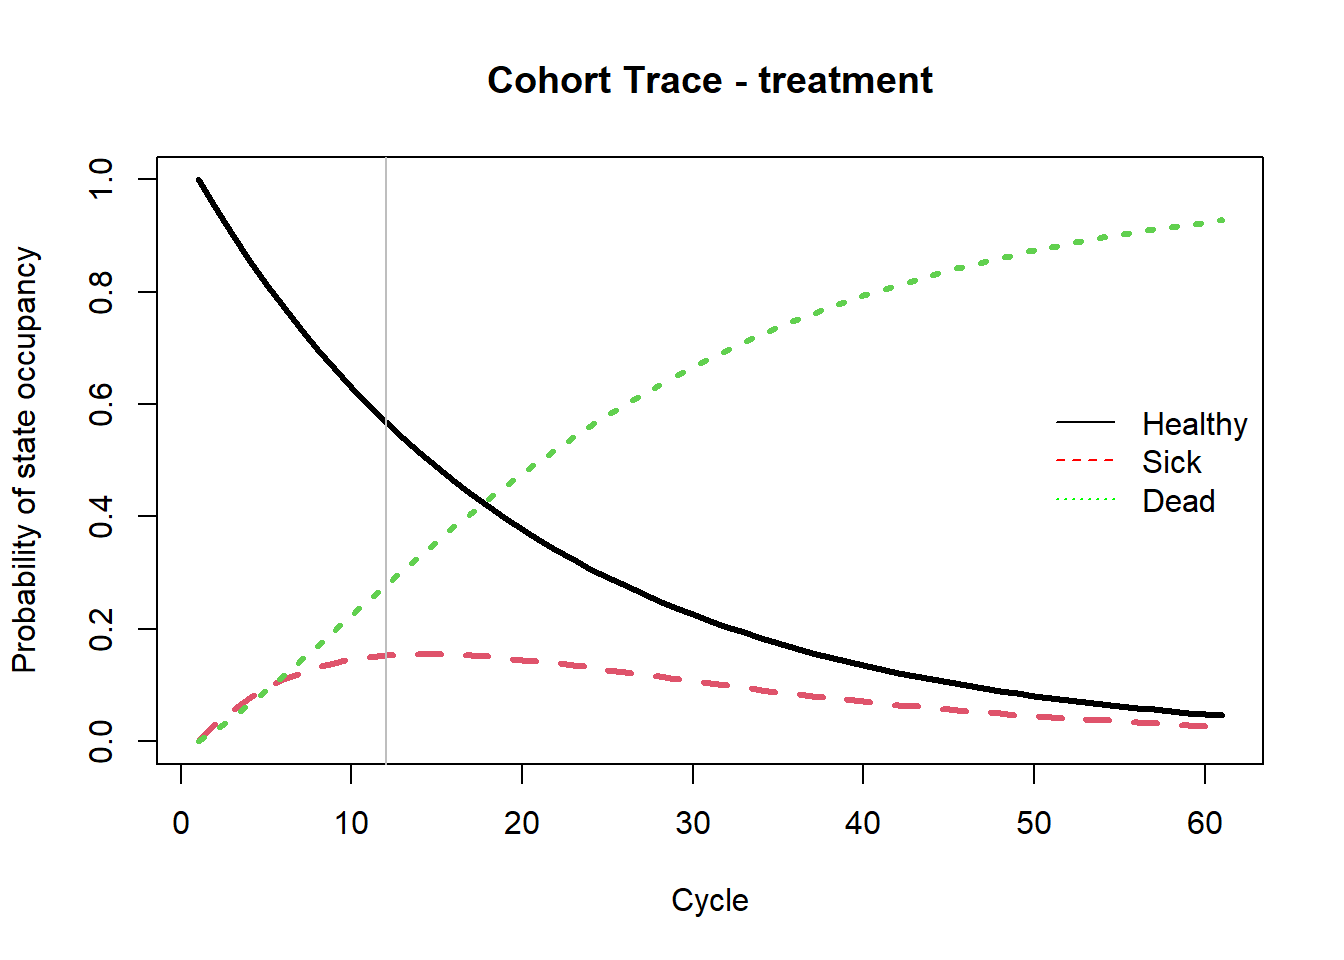
\includegraphics{Markov_3state_tunnels_files/figure-latex/unnamed-chunk-11-1.pdf}

\hypertarget{overall-survival-os}{%
\subsection{06.2 Overall Survival (OS)}\label{overall-survival-os}}

\begin{Shaded}
\begin{Highlighting}[]
\NormalTok{v_os <-}\StringTok{ }\DecValTok{1} \OperatorTok{-}\StringTok{ }\NormalTok{m_M_tunnels[, }\StringTok{"Dead"}\NormalTok{]    }\CommentTok{# calculate the overall survival (OS) probability}
\NormalTok{v_os <-}\StringTok{ }\KeywordTok{rowSums}\NormalTok{(m_M_tunnels[, }\DecValTok{1}\OperatorTok{:}\DecValTok{2}\NormalTok{])  }\CommentTok{# alternative way of calculating the OS probability   }

\CommentTok{# create a simple plot showing the OS}
\KeywordTok{plot}\NormalTok{(v_os, }\DataTypeTok{type =} \StringTok{'l'}\NormalTok{, }
     \DataTypeTok{ylim =} \KeywordTok{c}\NormalTok{(}\DecValTok{0}\NormalTok{, }\DecValTok{1}\NormalTok{),}
     \DataTypeTok{ylab =} \StringTok{"Survival probability"}\NormalTok{,}
     \DataTypeTok{xlab =} \StringTok{"Cycle"}\NormalTok{,}
     \DataTypeTok{main =} \StringTok{"Overall Survival"}\NormalTok{)             }
\CommentTok{# add grid }
\KeywordTok{grid}\NormalTok{(}\DataTypeTok{nx =}\NormalTok{ n_t, }\DataTypeTok{ny =} \DecValTok{10}\NormalTok{, }\DataTypeTok{col =} \StringTok{"lightgray"}\NormalTok{, }\DataTypeTok{lty =} \StringTok{"dotted"}\NormalTok{, }\DataTypeTok{lwd =} \KeywordTok{par}\NormalTok{(}\StringTok{"lwd"}\NormalTok{), }\DataTypeTok{equilogs =} \OtherTok{TRUE}\NormalTok{) }
\end{Highlighting}
\end{Shaded}

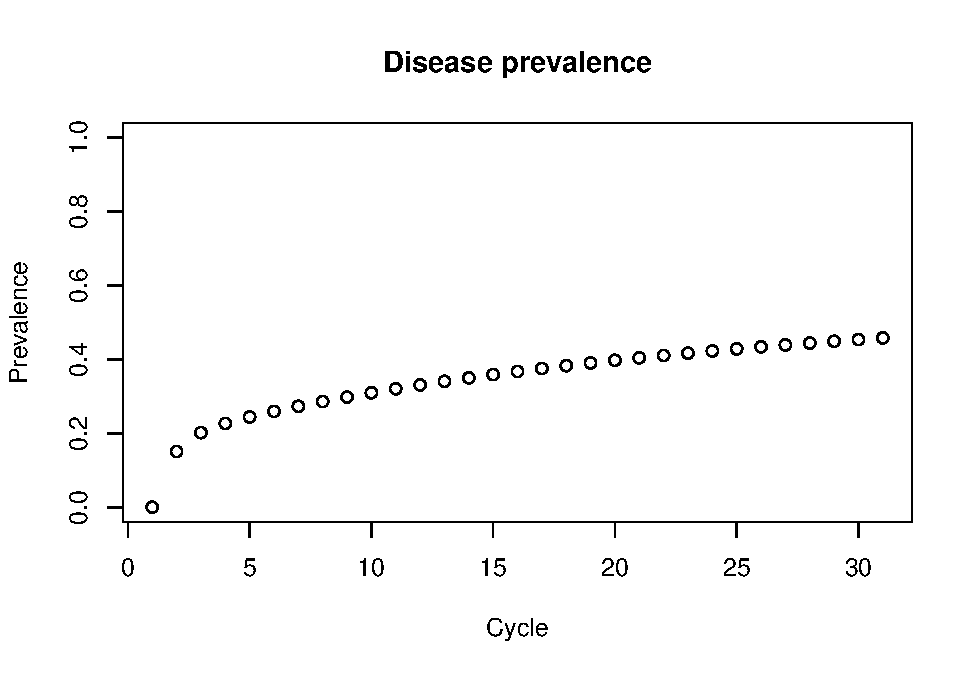
\includegraphics{Markov_3state_tunnels_files/figure-latex/unnamed-chunk-12-1.pdf}

\hypertarget{life-expectancy-le}{%
\subsection{06.2.1 Life Expectancy (LE)}\label{life-expectancy-le}}

\begin{Shaded}
\begin{Highlighting}[]
\NormalTok{v_le <-}\StringTok{ }\KeywordTok{sum}\NormalTok{(v_os)           }\CommentTok{# summing probablity of OS over time  (i.e. life expectancy)}
\end{Highlighting}
\end{Shaded}

\hypertarget{disease-prevalence}{%
\subsection{06.3 Disease prevalence}\label{disease-prevalence}}

\begin{Shaded}
\begin{Highlighting}[]
\NormalTok{v_prev <-}\StringTok{ }\NormalTok{m_M_tunnels[, }\StringTok{"Sick"}\NormalTok{]}\OperatorTok{/}\NormalTok{v_os}
\KeywordTok{plot}\NormalTok{(v_prev,}
     \DataTypeTok{ylim =} \KeywordTok{c}\NormalTok{(}\DecValTok{0}\NormalTok{, }\DecValTok{1}\NormalTok{),}
     \DataTypeTok{ylab =} \StringTok{"Prevalence"}\NormalTok{,}
     \DataTypeTok{xlab =} \StringTok{"Cycle"}\NormalTok{,}
     \DataTypeTok{main =} \StringTok{"Disease prevalence"}\NormalTok{)}
\end{Highlighting}
\end{Shaded}

\includegraphics{Markov_3state_tunnels_files/figure-latex/unnamed-chunk-14-1.pdf}

\hypertarget{compute-cost-effectiveness-outcomes}{%
\section{07 Compute Cost-Effectiveness
Outcomes}\label{compute-cost-effectiveness-outcomes}}

\hypertarget{mean-costs-and-qalys}{%
\subsection{07.1 Mean Costs and QALYs}\label{mean-costs-and-qalys}}

\begin{Shaded}
\begin{Highlighting}[]
\CommentTok{# per cycle}
\CommentTok{# calculate expected costs by multiplying m_M with the cost vector for the different }
\CommentTok{# health states   }
\NormalTok{v_tc <-}\StringTok{ }\NormalTok{m_M_tunnels }\OperatorTok\StringTok{ }\KeywordTok{c}\NormalTok{(c_H, c_S, c_D)  }
\CommentTok{# calculate expected QALYs by multiplying m_M with the utilities for the different }
\CommentTok{# health states   }
\NormalTok{v_tu <-}\StringTok{ }\NormalTok{m_M_tunnels }\OperatorTok\StringTok{ }\KeywordTok{c}\NormalTok{(u_H, u_S, u_D)  }
\end{Highlighting}
\end{Shaded}

\hypertarget{discounted-mean-costs-and-qalys}{%
\subsection{07.2 Discounted Mean Costs and
QALYs}\label{discounted-mean-costs-and-qalys}}

\begin{Shaded}
\begin{Highlighting}[]
\CommentTok{# Discount costs  by multiplying the cost vector with discount weights (v_dw) }
\NormalTok{v_tc_d <-}\StringTok{  }\KeywordTok{t}\NormalTok{(v_tc) }\OperatorTok\StringTok{ }\NormalTok{v_dwc}
\CommentTok{# Discount QALYS  by multiplying the QALYs vector with discount weights (v_dw)}
\NormalTok{v_te_d <-}\StringTok{  }\KeywordTok{t}\NormalTok{(v_tu) }\OperatorTok\StringTok{ }\NormalTok{v_dwe}
\end{Highlighting}
\end{Shaded}

\hypertarget{results}{%
\subsection{07.3 Results}\label{results}}

\begin{Shaded}
\begin{Highlighting}[]
\NormalTok{results <-}\StringTok{ }\KeywordTok{data.frame}\NormalTok{( }\StringTok{"Total Discounted Cost"}\NormalTok{ =}\StringTok{ }\NormalTok{v_tc_d, }
                       \StringTok{"Life Expectancy"}\NormalTok{ =}\StringTok{ }\NormalTok{v_le, }
                       \StringTok{"Total Discounted QALYs"}\NormalTok{ =}\StringTok{ }\NormalTok{v_te_d, }
                       \DataTypeTok{check.names =}\NormalTok{ F)}
\NormalTok{results}
\end{Highlighting}
\end{Shaded}

\begin{verbatim}
##   Total Discounted Cost Life Expectancy Total Discounted QALYs
## 1              9382.938        25.89709               11.98968
\end{verbatim}

\end{document}
